% !TeX program = xelatex
\documentclass[a4paper,10pt]{article}

% ============================================================================
% កញ្ចប់បណ្ណាល័យ (Packages) – តាមលំនាំ NGS Preah Krasang (ls_plan.tex)
% បរិបទ៖ គ្មានស្លាយ LCD និងគ្មានម៉ាស៊ីនគិតលេខ — ប្រើសន្លឹកកិច្ចការសិស្ស (ស-ខ្មៅ) និងក្ដារខៀនជាគោល
% ============================================================================
\usepackage[a4paper, left=0.95cm, right=0.95cm, top=0.85cm, bottom=0.92cm, footskip=0.52cm]{geometry}
\usepackage{amsmath}
\usepackage{unicode-math}
\usepackage{fontspec}
\usepackage{array, longtable, multirow, colortbl}
\usepackage[table]{xcolor}
\usepackage{enumitem}
\usepackage{pifont}
\usepackage{fancyhdr}
\usepackage{tikz}
\usetikzlibrary{calc, arrows.meta, angles, quotes, decorations.markings, decorations.pathreplacing, patterns, babel}

\makeatletter
\let\@expl@@@mark@update@singlecol@structures@@\relax
\makeatother

\providecommand{\NGSFindFonts}{%
  \IfFileExists{C:/Windows/Fonts/cambria.ttc}{%
    \def\NGSSysPath{C:/Windows/Fonts/}%
    \def\NGSUserPath{C:/Users/KIT/AppData/Local/Microsoft/Windows/Fonts/}%
  }{%
    \IfFileExists{./fonts/KhmerOSsiemreap.ttf}{\def\NGSSysPath{./fonts/}\def\NGSUserPath{./fonts/}}{%
    \IfFileExists{../fonts/KhmerOSsiemreap.ttf}{\def\NGSSysPath{../fonts/}\def\NGSUserPath{../fonts/}}{%
    \IfFileExists{../../fonts/KhmerOSsiemreap.ttf}{\def\NGSSysPath{../../fonts/}\def\NGSUserPath{../../fonts/}}{%
    \IfFileExists{../../../fonts/KhmerOSsiemreap.ttf}{\def\NGSSysPath{../../../fonts/}\def\NGSUserPath{../../../fonts/}}{%
    \IfFileExists{../../../../fonts/KhmerOSsiemreap.ttf}{\def\NGSSysPath{../../../../fonts/}\def\NGSUserPath{../../../../fonts/}}{%
    \IfFileExists{../../../../../fonts/KhmerOSsiemreap.ttf}{\def\NGSSysPath{../../../../../fonts/}\def\NGSUserPath{../../../../../fonts/}}{%
    \IfFileExists{../../../../../../fonts/KhmerOSsiemreap.ttf}{\def\NGSSysPath{../../../../../../fonts/}\def\NGSUserPath{../../../../../../fonts/}}{%
      \def\NGSSysPath{../../../../../../../fonts/}\def\NGSUserPath{../../../../../../../fonts/}%
    }}}}}}}%
  }%
}
\NGSFindFonts

\setmathfont[Path={\NGSSysPath}, FontIndex=1, Scale=1.02]{cambria.ttc}
\defaultfontfeatures{Ligatures=TeX}

\setmainfont[
  Path={\NGSUserPath}, Extension=.ttf, Script=Khmer,
  BoldFont={KhmerOSsiemreap}, BoldFeatures={FakeBold=1.8},
  ItalicFont={KhmerOSsiemreap}, ItalicFeatures={FakeSlant=0.25},
  BoldItalicFont={KhmerOSsiemreap}, BoldItalicFeatures={FakeBold=1.8, FakeSlant=0.25}
]{KhmerOSsiemreap}

\newfontfamily\muol[Path={\NGSUserPath}, Extension=.ttf, Script=Khmer]{KhmerOSmuollight}
\newfontfamily\TimesEn[Path={\NGSSysPath}, Extension=.ttf, Scale=1.00, BoldFont={timesbd}, ItalicFont={timesi}, BoldItalicFont={timesbi}]{times}
\newfontfamily\NagaBold[Path={\NGSUserPath}, Extension=.ttf]{AKbalthom Naga Bold}
\newfontfamily\CalibriFont[Path={\NGSSysPath}, Extension=.ttf]{calibri}
\newfontfamily\Tacteing[Path={\NGSUserPath}]{TACTENG.TTF}
\newfontfamily\CourierBullet[Path={\NGSSysPath}, Extension=.ttf]{cour}
\newcommand{\wcirc}{{\CourierBullet\fontsize{9.5pt}{11pt}\selectfont o}}

\XeTeXlinebreaklocale "km"
\XeTeXlinebreakskip = 0pt plus 1pt minus 0.1pt

\definecolor{stepgray}{HTML}{D9D9D9}
\definecolor{headgray}{HTML}{F2F2F2}
\definecolor{boxgray}{HTML}{D9D9D9}
\definecolor{darkred}{HTML}{C00000}
\definecolor{red5e}{HTML}{FF0000}

\pagestyle{fancy}
\fancyhf{}
\renewcommand{\headrulewidth}{0pt}
\fancyfoot[R]{\CalibriFont\fontsize{11pt}{13pt}\selectfont\thepage}

\setlength{\parindent}{0pt}
\setlength{\parskip}{0pt}
\setlength{\tabcolsep}{3.8pt}

\newcolumntype{L}[1]{>{\raggedright\arraybackslash}p{#1}}
\newcolumntype{C}[1]{>{\centering\arraybackslash}p{#1}}

\newcommand{\en}[1]{{\TimesEn #1}}
\newcommand{\enbf}[1]{{\TimesEn\textbf{#1}}}
\newcommand{\unit}[1]{\,\text{\en{#1}}}
\newcommand{\fiveE}[1]{{\NagaBold\fontsize{9.5pt}{13pt}\selectfont\textcolor{red5e}{#1}}}
\newcommand{\timenote}[1]{\textcolor{darkred}{\textit{#1}}}
\newcommand{\redsub}[1]{\textcolor{darkred}{#1}}
\newcommand{\graybox}[1]{\colorbox{boxgray}{\strut\hspace{2pt}#1\hspace{2pt}}}
\newcommand{\ditem}{\tikz[baseline=-0.5ex]\fill (0,0.42ex) -- (0.42ex,0) -- (0,-0.42ex) -- (-0.42ex,0) -- cycle;\hspace{0.3em}}
\newcommand{\cnum}[1]{{\fontsize{10.5pt}{12pt}\selectfont\ding{\numexpr181+#1\relax}}\hspace{0.15em}}
\newcommand{\cfig}[1]{\par\vspace{3pt}{\centering #1\par}\vspace{3pt}}
\newcommand{\stepheader}[1]{\multicolumn{3}{|c|}{\cellcolor{stepgray}\muol #1} \\* \noalign{\hrule height 0.4pt}}
\newcommand{\khmflourish}{{\Tacteing\fontsize{36pt}{14pt}\selectfont\raisebox{-5pt}{3}}}

% ============================================================================
% ម៉ាក្រូគូសរូប TikZ ស-ខ្មៅ ១០០% សម្រាប់មេរៀន ៣.២.៥ ការប្រាក់សាមញ្ញ (SINT)
% ============================================================================

% ១. E1 Engage: អន្ទាក់ការប្រាក់សាមញ្ញច្រើនឆ្នាំ និងអន្ទាក់រយៈពេលគិតជាខែ
\newcommand{\figEngageSINT}{%
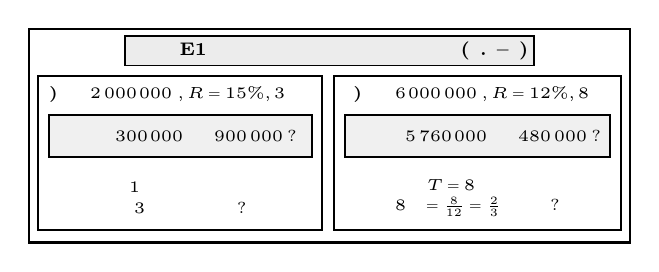
\begin{tikzpicture}[x=0.96cm, y=0.92cm, every node/.style={font=\scriptsize, text=black}]
  \draw[black, line width=0.95pt] (0,0) rectangle (7.95,2.95);
  \node[fill=gray!15, draw=black, line width=0.6pt, inner sep=2pt, font=\fontsize{6.6pt}{8.4pt}\selectfont\bfseries] at (3.975,2.65) {បេសកកម្ម \en{E1}៖ ប្រាក់បញ្ញើធនាគារ និងច្រកប្ដូររយៈពេលខែជាឆ្នាំ (ទំ.៣៥–៣៦)};

  \draw[black, line width=0.8pt] (0.12,0.18) rectangle (3.88,2.30);
  \node[font=\fontsize{5.8pt}{7.5pt}\selectfont\bfseries] at (2.00,2.04) {១) ដាក់ $2\,000\,000\text{៛}, R=15\%, 3$ ឆ្នាំ};
  \draw[black, line width=0.75pt, fill=gray!12] (0.26,1.18) rectangle (3.74,1.76);
  \node[font=\fontsize{5.8pt}{7.5pt}\selectfont] at (2.00,1.47) {ការប្រាក់៖ $300\,000\text{៛}$ \;ឬ\; $900\,000\text{៛}$?};
  \node[align=center, font=\fontsize{5.8pt}{7.4pt}\selectfont] at (2.00,0.62) {ក្នុង $1$ ឆ្នាំបានការប្រាក់ស្មើគ្នា\\ចុះ $3$ ឆ្នាំគុណនឹងប៉ុន្មាន?};

  \draw[black, line width=0.8pt] (4.04,0.18) rectangle (7.83,2.30);
  \node[font=\fontsize{5.8pt}{7.5pt}\selectfont\bfseries] at (5.935,2.04) {២) ខ្ចី $6\,000\,000\text{៛}, R=12\%, 8$ ខែ};
  \draw[black, line width=0.75pt, fill=gray!12] (4.18,1.18) rectangle (7.69,1.76);
  \node[font=\fontsize{5.8pt}{7.5pt}\selectfont] at (5.935,1.47) {ការប្រាក់៖ $5\,760\,000\text{៛}$ \;ឬ\; $480\,000\text{៛}$?};
  \node[align=center, font=\fontsize{5.8pt}{7.4pt}\selectfont] at (5.935,0.62) {តើជំនួស $T=8$ ត្រង់ៗ ឬត្រូវប្ដូរ\\$8\text{ ខែ} = \frac{8}{12} = \frac{2}{3}\text{ ឆ្នាំ}$ សិន?};
\end{tikzpicture}}

% ២. E2 POE 2: ច្រកប្ដូរខែជាឆ្នាំ និងត្រីកោណទាញរកអញ្ញាត P-R-T-I
\newcommand{\figGateSINT}{%
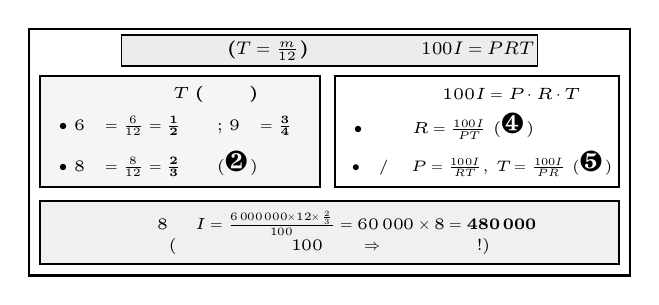
\begin{tikzpicture}[x=0.96cm, y=0.92cm, every node/.style={font=\scriptsize, text=black}]
  \draw[black, line width=0.95pt] (0,0) rectangle (7.95,3.40);
  \node[fill=gray!15, draw=black, line width=0.6pt, inner sep=2pt, font=\fontsize{6.6pt}{8.4pt}\selectfont\bfseries] at (3.975,3.10) {ច្រកប្ដូរខែជាឆ្នាំ ($T = \frac{m}{12}$) និងការទាញរកអញ្ញាតពី $100 I = P R T$};

  % Left box: Month-to-Year gate
  \draw[black, line width=0.8pt, fill=gray!8] (0.15,1.22) rectangle (3.85,2.75);
  \node[font=\fontsize{5.9pt}{7.5pt}\selectfont\bfseries] at (2.00,2.50) {ច្រកឯកតារយៈពេល $T$ (គិតជាឆ្នាំ)};
  \node[anchor=west, font=\fontsize{5.8pt}{7.4pt}\selectfont] at (0.28,2.06) {$\bullet$ $6\text{ ខែ} = \frac{6}{12} = \mathbf{\frac{1}{2}\text{ ឆ្នាំ}}$ ; $9\text{ ខែ} = \mathbf{\frac{3}{4}\text{ ឆ្នាំ}}$};
  \node[anchor=west, font=\fontsize{5.8pt}{7.4pt}\selectfont] at (0.28,1.54) {$\bullet$ $8\text{ ខែ} = \frac{8}{12} = \mathbf{\frac{2}{3}\text{ ឆ្នាំ}}$ (\cnum{2})};

  % Right box: Inverse formulas
  \draw[black, line width=0.8pt] (4.05,1.22) rectangle (7.80,2.75);
  \node[font=\fontsize{5.9pt}{7.5pt}\selectfont\bfseries] at (5.925,2.50) {បំប្លែងសមីការ $100 I = P \cdot R \cdot T$};
  \node[anchor=west, font=\fontsize{5.8pt}{7.4pt}\selectfont] at (4.18,2.06) {$\bullet$ រកអត្រា៖ $R = \frac{100 I}{P T}$ (\cnum{4})};
  \node[anchor=west, font=\fontsize{5.5pt}{7.2pt}\selectfont] at (4.15,1.54) {$\bullet$ ដើម/ពេល៖ $P=\frac{100 I}{R T},\; T=\frac{100 I}{P R}$ (\cnum{5})};

  % Bottom example bar
  \draw[black, line width=0.75pt, fill=gray!12] (0.15,0.16) rectangle (7.80,1.02);
  \node[align=center, font=\fontsize{5.8pt}{7.5pt}\selectfont] at (3.975,0.59) {\textbf{ឧទាហរណ៍ $8$ ខែ៖} $I = \frac{6\,000\,000 \times 12 \times \frac{2}{3}}{100} = 60\,000 \times 8 = \mathbf{480\,000\text{៛}}$\\(សម្រួលសូន្យពីរខ្ទង់ជាមួយ $100$ មុនគុណ $\Rightarrow$ គណនាដោយដៃរហ័សឥតខ្ចោះ!)};
\end{tikzpicture}}

% ៣. E4 Worked Example: គំរូមីងផុន (ទំ.៣៦ ទាំង ក និង ខ — កែតម្រូវកំហុសបោះពុម្ព)
\newcommand{\figMingPhonSINT}{%
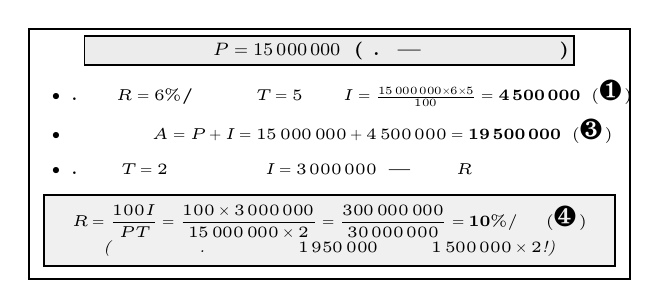
\begin{tikzpicture}[x=0.96cm, y=0.92cm, every node/.style={font=\scriptsize, text=black}]
  \draw[black, line width=0.95pt] (0,0) rectangle (7.95,3.45);
  \node[fill=gray!15, draw=black, line width=0.6pt, inner sep=2pt, font=\fontsize{6.5pt}{8.3pt}\selectfont\bfseries] at (3.975,3.15) {គំរូមីងផុនដាក់ប្រាក់ដើម $P = 15\,000\,000\text{៛}$ (ទំ.៣៦ — កែលេខបោះពុម្ពឱ្យត្រឹមត្រូវ)};

  \node[anchor=west, font=\fontsize{5.7pt}{7.4pt}\selectfont] at (0.18,2.56) {$\bullet$ \textbf{ក. អត្រា $R = 6\%$/ឆ្នាំ រយៈពេល $T = 5$ ឆ្នាំ៖} $I = \frac{15\,000\,000\times 6\times 5}{100} = \mathbf{4\,500\,000\text{៛}}$ (\cnum{1})};
  \node[anchor=west, font=\fontsize{5.7pt}{7.4pt}\selectfont] at (0.18,2.04) {$\bullet$ \textbf{ប្រាក់សរុបចុងគ្រា៖} $A = P + I = 15\,000\,000 + 4\,500\,000 = \mathbf{19\,500\,000\text{៛}}$ (\cnum{3})};
  \node[anchor=west, font=\fontsize{5.7pt}{7.4pt}\selectfont] at (0.18,1.52) {$\bullet$ \textbf{ខ. រយៈពេល $T = 2$ ឆ្នាំ បានការប្រាក់ $I = 3\,000\,000\text{៛}$ — រកអត្រា $R$៖}};

  \draw[black, line width=0.75pt, fill=gray!12] (0.20,0.18) rectangle (7.75,1.16);
  \node[align=center, font=\fontsize{5.7pt}{7.4pt}\selectfont] at (3.975,0.67) {$R = \dfrac{100 I}{P T} = \dfrac{100 \times 3\,000\,000}{15\,000\,000 \times 2} = \dfrac{300\,000\,000}{30\,000\,000} = \mathbf{10\%}\text{/ឆ្នាំ}$ (\cnum{4})\\\textit{(កែតម្រូវសៀវភៅពុម្ពទំ.៣៦ ដែលបោះពុម្ពច្រឡំ $1\,950\,000$ និងភាគបែង $1\,500\,000\times 2$!)}};
\end{tikzpicture}}

% ៤. E5 Diagnostic Options A-D
\newcommand{\figExitCardsSINT}{%
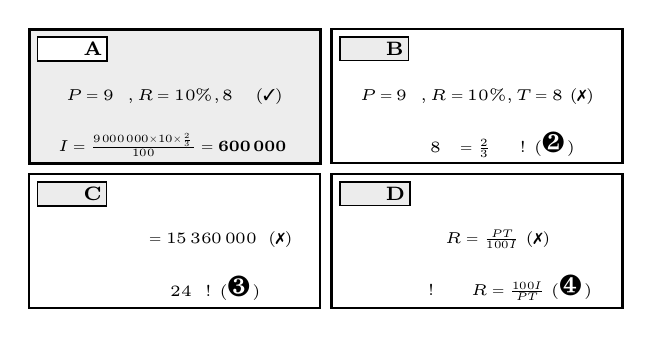
\begin{tikzpicture}[x=0.96cm, y=0.92cm, every node/.style={font=\scriptsize, text=black}]
  \draw[black, line width=1.1pt, fill=gray!14] (0,2.00) rectangle (3.85,3.85);
  \node[anchor=north west, fill=white, draw=black, line width=0.6pt, inner sep=1.8pt] at (0.10,3.75) {\textbf{ជម្រើស \en{A}}};
  \node[font=\fontsize{5.7pt}{7.4pt}\selectfont] at (1.925,2.92) {$P=9\text{លាន}, R=10\%, 8\text{ ខែ}$ (\ding{51})};
  \node[font=\fontsize{5.7pt}{7.4pt}\selectfont] at (1.925,2.25) {$I = \frac{9\,000\,000\times 10\times \frac{2}{3}}{100} = \mathbf{600\,000\text{៛}}$};

  \draw[black, line width=0.9pt] (4.00,2.00) rectangle (7.85,3.85);
  \node[anchor=north west, fill=gray!15, draw=black, line width=0.6pt, inner sep=1.8pt] at (4.10,3.75) {\textbf{ជម្រើស \en{B}}};
  \node[font=\fontsize{5.7pt}{7.4pt}\selectfont] at (5.925,2.92) {$P=9\text{លាន}, R=10\%, T=8$ (\ding{55})};
  \node[font=\fontsize{5.7pt}{7.4pt}\selectfont] at (5.925,2.25) {ភ្លេចប្ដូរ $8\text{ ខែ}=\frac{2}{3}\text{ ឆ្នាំ}$! (\cnum{2})};

  \draw[black, line width=0.9pt] (0,0) rectangle (3.85,1.85);
  \node[anchor=north west, fill=gray!15, draw=black, line width=0.6pt, inner sep=1.8pt] at (0.10,1.75) {\textbf{ជម្រើស \en{C}}};
  \node[font=\fontsize{5.7pt}{7.4pt}\selectfont] at (1.925,0.95) {ជីកទ្រី៖ ប្រាក់សរុប $= 15\,360\,000\text{៛}$ (\ding{55})};
  \node[font=\fontsize{5.7pt}{7.4pt}\selectfont] at (1.925,0.28) {ភ្លេចបូកប្រាក់ដើម $24\text{លាន}$! (\cnum{3})};

  \draw[black, line width=0.9pt] (4.00,0) rectangle (7.85,1.85);
  \node[anchor=north west, fill=gray!15, draw=black, line width=0.6pt, inner sep=1.8pt] at (4.10,1.75) {\textbf{ជម្រើស \en{D}}};
  \node[font=\fontsize{5.7pt}{7.4pt}\selectfont] at (5.925,0.95) {រកអត្រា៖ $R = \frac{PT}{100 I}$ (\ding{55})};
  \node[font=\fontsize{5.7pt}{7.4pt}\selectfont] at (5.925,0.28) {ច្រាសរូបមន្តខុស! ត្រូវ $R=\frac{100I}{PT}$ (\cnum{4})};
\end{tikzpicture}}

\begin{document}
\fontsize{10pt}{15.2pt}\selectfont

% -------------------- ក្បាលកិច្ចតែងការ --------------------
\begin{center}
  {\muol\fontsize{11pt}{16pt}\selectfont ព្រះរាជាណាចក្រកម្ពុជា}\\[2pt]
  {\muol\fontsize{10pt}{15pt}\selectfont ជាតិ សាសនា ព្រះមហាក្សត្រ}\\[1pt]
  \khmflourish
\end{center}

\vspace{-24pt}
{\muol\fontsize{9.5pt}{12.5pt}\selectfont
មន្ទីរអប់រំ យុវជន និងកីឡា ខេត្តកំពង់ធំ\\
ការិយាល័យអប់រំ យុវជន និងកីឡា ស្រុកកំពង់ស្វាយ\\
អនុវិទ្យាល័យព្រះក្រសាំង}

\vspace{1pt}
\begin{center}
  {\muol\fontsize{10pt}{14pt}\selectfont កិច្ចតែងការបង្រៀន}
\end{center}
\vspace{0pt}

% -------------------- ព័ត៌មានទូទៅ --------------------
{\renewcommand{\arraystretch}{0.98}
\hspace*{3.1cm}%
\begin{tabular}{@{}l l L{11.0cm}@{}}
  - \hspace{0.35cm} មុខវិជ្ជា & : & គណិតវិទ្យា ថ្នាក់ទី៨ (ពីជគណិត) \\
  - \hspace{0.35cm} ចំណងជើងមេរៀន & : & មេរៀនទី៣៖ ទំហំសមាមាត្រ និងភាគរយ \\
  - \hspace{0.35cm} ចំណងជើងរង & : & ២.៥. ការប្រាក់សាមញ្ញ ($I = \dfrac{PRT}{100}$, ទំ.៣៥–៣៧ និង \#16 ទំ.៤២) \\
  - \hspace{0.35cm} រយៈពេល & : & ១ ម៉ោងសិក្សា (៥០ នាទី) \\
  - \hspace{0.35cm} បង្រៀនដោយ & : & ហុក ប៊ុនថែន \\
  - \hspace{0.35cm} កាលបរិច្ឆេទ & : & ថ្ងៃអង្គារ ទី១ ខែធ្នូ ឆ្នាំ២០២៦ \\
\end{tabular}

\vspace{2pt}

% -------------------- I. វត្ថុបំណង --------------------
\textbf{I.} {\muol វត្ថុបំណង}\\[1pt]
\hspace*{0.55cm}%
\begin{tabular}{@{}l l L{14.2cm}@{}}
  \wcirc \hspace{0.25cm} វិជ្ជាសម្បទា & : & សិស្សប្រាប់និយមន័យ និងរូបមន្តការប្រាក់សាមញ្ញ $I = \dfrac{PRT}{100}$ ប្រាក់សរុប $A = P + I$ និងរូបមន្តច្រាសរក $R, T, P$ បានត្រឹមត្រូវ ។ \\
  \wcirc \hspace{0.25cm} បំណិនសម្បទា & : & សិស្សគណនាការប្រាក់សាមញ្ញ ប្រាក់សរុប អត្រាការប្រាក់ និងប្ដូររយៈពេលខែជាប្រភាគនៃឆ្នាំ ($T = \frac{m}{12}$) ដោយដៃលើសន្លឹកកិច្ចការបានស្ទាត់ជំនាញ ។ \\
  \wcirc \hspace{0.25cm} ចរិយាសម្បទា & : & សិស្សមានទម្លាប់សន្សំសំចៃ និងពិនិត្យលក្ខខណ្ឌអត្រាការប្រាក់ប្រចាំឆ្នាំព្រមទាំងរយៈពេលកម្ចី-បញ្ញើក្នុងជីវភាពរស់នៅដោយប្រុងប្រយ័ត្ន ។ \\
\end{tabular}

\vspace{2pt}

% -------------------- II. សម្ភារៈឧបទេស --------------------
\textbf{II.} {\muol សម្ភារៈឧបទេស}\\[1pt]
\hspace*{0.55cm}$\bullet$ \hspace{0.35cm} សៀវភៅសិក្សាគោលគណិតវិទ្យាថ្នាក់ទី៨ (ទំ.៣៥–៣៧, ៤២) ក្ដារខៀន ដីស និងសន្លឹកកិច្ចការសិស្ស ស-ខ្មៅ (\en{Worksheet\_SINT} ទំព័រ ១–២ គ្មានស្លាយ \en{LCD})

\vspace{2pt}

% -------------------- III. វិធីសាស្រ្តបង្រៀន --------------------
\textbf{III.} {\muol វិធីសាស្រ្តបង្រៀន}\\[1pt]
\hspace*{0.45cm}%
\begin{tabular}{@{}l l L{14.85cm}@{}}
  $\bullet$ \hspace{0.25cm} គោលវិធី & : & សិស្សមជ្ឈមណ្ឌល (បង្រៀនតាមសន្លឹកកិច្ចការស៊ើបអង្កេត និងក្ដារខៀន គ្មាន \en{LCD}) \\
  $\bullet$ \hspace{0.25cm} យុទ្ធវិធីបង្រៀន & : & គំរូ \en{5Es} រួមបញ្ចូលតារាងបំបែកអញ្ញាត $P\text{-}R\text{-}T\text{-}I$ និងច្រកប្ដូរខែជាប្រភាគនៃឆ្នាំ (\en{Month-to-Year Gate}) \\
\end{tabular}
}

\vspace{2pt}

% -------------------- IV. ដំណើរការបង្រៀន --------------------
\textbf{IV.} {\muol ដំណើរការបង្រៀន}

\vspace{1pt}

\renewcommand{\arraystretch}{1.15}
\begin{longtable}{|L{5.50cm}|L{7.90cm}|L{4.80cm}|}
\hline
\rowcolor{headgray}
\multicolumn{1}{|c|}{\muol សកម្មភាពគ្រូ} &
\multicolumn{1}{c|}{\muol ខ្លឹមសារមេរៀន} &
\multicolumn{1}{c|}{\muol សកម្មភាពសិស្ស} \\
\hline
\endfirsthead
\hline
\endhead
\hline
\endfoot
\hline
\endlastfoot

% ==================== ជំហានទី១ (2min) ====================
\stepheader{ជំហានទី១ \enbf{(}រដ្ឋបាលថ្នាក់\enbf{)}}
$\bullet$ ពិនិត្យអវត្តមាន អនាម័យ និងសណ្ដាប់ធ្នាប់ថ្នាក់រៀន
&
$\bullet$ រដ្ឋបាលថ្នាក់ និងការរៀបចំដៃគូសិក្សា
&
$\circ$ ប្រធានថ្នាក់រាយការណ៍អវត្តមាន \\[3pt]

$\bullet$ ចែក \textbf{សន្លឹកកិច្ចការសិស្ស (\en{Worksheet\_SINT})} ម្នាក់ ១ សន្លឹក (ផ្កាប់ទុកសិន)
&
$\bullet$ សន្លឹកកិច្ចការសិស្ស ស-ខ្មៅ (\en{Worksheet\_SINT} ទំព័រ ១–២)
&
$\circ$ ទទួលសន្លឹកកិច្ចការ និងត្រៀមសម្ភារៈសរសេរ \\
\hline

% ==================== ជំហានទី២ (9min: <=3 + 3 + E1 3) ====================
\stepheader{ជំហានទី២ \enbf{(}កិច្ចការផ្ទះ \enbf{+} ទំនាក់ទំនងមេរៀនថ្មី\enbf{)}}
\ditem \textbf{កំណែកិច្ចការផ្ទះ ($\le 3\unit{min}$)} \timenote{(កុំសរសេរវែង)} \par
$\bullet$ ហៅសិស្ស ២ នាក់ឡើងសរសេរចម្លើយលំហាត់ \#14 និង \#15 (ទំ.៤១–៤២) លើក្ដារខៀន
&
{\centering\redsub{កំណែកិច្ចការផ្ទះមេរៀន ២.៣–២.៤ (ទំ.៤១–៤២ \#14, \#15)}\par} \par
$\bullet$ \textbf{\#14៖} គណនាភាគរយបញ្ចុះតម្លៃធៀបនឹងថ្លៃដាក់លក់ ($100\%$) \par
$\bullet$ \textbf{\#15៖} គណនាបម្រែបម្រួលភាគរយ និងរកតម្លៃដើមត្រឡប់ក្រោយតាម $\frac{100}{100\pm p}$
&
$\circ$ ផ្ទៀងផ្ទាត់ និងកែតម្រូវចម្លើយក្នុងសៀវភៅកិច្ចការផ្ទះ \\[3pt]

\ditem \textbf{រំលឹកមេរៀនទាក់ទង (3min)} \par
$\bullet$ សួររហ័ស៖ គណនា $15\%$ នៃ $2\,000\,000\text{៛}$ ដោយសម្រួលសូន្យពីរខ្ទង់
&
{\centering\redsub{រំលឹកភាគរយនៃប្រាក់ និងការប្ដូរខែជាប្រភាគនៃឆ្នាំ}\par} \par
$\bullet$ $15\%$ នៃ $2\,000\,000\text{៛} = 2\,000\,000 \times \dfrac{15}{100} = 20\,000\times 15 = \mathbf{300\,000\text{៛}}$
&
$\circ$ គណនារហ័សដោយសម្រួលសូន្យពីរខ្ទង់ជាមួយ $100$ \\[3pt]

$\bullet$ សួររហ័សបន្ត៖ ក្នុង $1$ ឆ្នាំមាន $12$ ខែ តើ $6$ ខែ និង $8$ ខែ ស្មើប៉ុន្មានប្រភាគនៃឆ្នាំ?
&
$\bullet$ $6\text{ ខែ} = \dfrac{6}{12} = \mathbf{\dfrac{1}{2}\text{ ឆ្នាំ}}$ \;;\; $8\text{ ខែ} = \dfrac{8}{12} = \mathbf{\dfrac{2}{3}\text{ ឆ្នាំ}}$
&
$\circ$ ឆ្លើយរហ័សថាស្មើ $\frac{1}{2}$ ឆ្នាំ និង $\frac{2}{3}$ ឆ្នាំ \\[3pt]

\fiveE{E1 - Engage (3min)} \timenote{(កុំទាន់ផ្ដល់ចម្លើយ)} \par
\ditem \textbf{«បេសកកម្មប្រាក់បញ្ញើធនាគារ និងអន្ទាក់រយៈពេលគិតជាខែ»} \par
$\bullet$ ឱ្យសិស្សបើកសន្លឹកកិច្ចការទំព័រ ១ គូសធីកទស្សន៍ទាយលើសំណួរ ២
&
{\centering\redsub{បេសកកម្ម E1៖ ការប្រាក់តាមឆ្នាំ និងអន្ទាក់ខែ-ឆ្នាំ}\par} \par
$\bullet$ \textbf{សំណួរ ១ (ទំ.៣៥)៖} ដាក់ប្រាក់ $2\,000\,000\text{៛}$ អត្រា $15\%$/ឆ្នាំ រយៈពេល $3$ ឆ្នាំ — តើការប្រាក់ស្មើ $300\,000\text{៛}$ ឬ $900\,000\text{៛}$? \par
$\bullet$ \textbf{សំណួរ ២៖} ខ្ចីប្រាក់ $6\,000\,000\text{៛}$ អត្រា $12\%$/ឆ្នាំ រយៈពេល $8$ ខែ — តើការប្រាក់ស្មើ $5\,760\,000\text{៛}$ ឬ $480\,000\text{៛}$?
&
$\circ$ គូសធីកទស្សន៍ទាយលើសន្លឹកកិច្ចការទំព័រ ១ \\[3pt]

&
\cfig{\figEngageSINT}
& \\[3pt]

$\bullet$ ស្រង់ចំនួនដៃសិស្សកត់លើក្ដារខៀន (មិនទាន់ប្រាប់ចម្លើយត្រូវ)
&
$\bullet$ ស្ថិតិទស្សន៍ទាយ៖ $300\,000\text{៛}$ ទល់នឹង $900\,000\text{៛}$ ; $5\,760\,000\text{៛}$ ទល់នឹង $480\,000\text{៛}$
&
$\circ$ លើកដៃបង្ហាញការទស្សន៍ទាយ \\
\hline

% ==================== ជំហានទី៣ (17min: E2 11m + E3 6m) ====================
\stepheader{ជំហានទី៣ \enbf{(}ខ្លឹមសារមេរៀនថ្មី\enbf{)}}
\fiveE{E2 - Explore (11min)} \par
$\bullet$ សរសេរចំណងជើងរងលើក្ដារខៀន
&
\textbf{២.៥. ការប្រាក់សាមញ្ញ} (សៀវភៅពុម្ព ទំ.៣៥–៣៧)
&
$\circ$ កត់ចំណងជើងចូលសៀវភៅ \\[3pt]

\ditem \textbf{សកម្មភាព ១៖ កសាងរូបមន្ត $I = \frac{PRT}{100}$ ពីកំណើនថេរប្រចាំឆ្នាំ \en{POE 1} (5min, ទំ.៣៥)} \par
$\bullet$ ឱ្យដៃគូបំពេញតារាងការប្រាក់នៃប្រាក់ដើម $P = 2\,000\,000\text{៛}$ អត្រា $R = 15\%$/ឆ្នាំ សម្រាប់ $1$ ឆ្នាំ, $2$ ឆ្នាំ, និង $3$ ឆ្នាំ លើសន្លឹកកិច្ចការ
&
{\centering\textbf{សកម្មភាព ១ (\en{POE 1})៖ ពីការប្រាក់ $1$ ឆ្នាំ ទៅ $T$ ឆ្នាំ (ទំ.៣៥)}\par} \par
$\bullet$ $1$ ឆ្នាំ៖ $2\,000\,000\times \dfrac{15}{100} = 300\,000\text{៛}$ \par
$\bullet$ $3$ ឆ្នាំ៖ $\dfrac{2\,000\,000\times 15\times 3}{100} = \mathbf{900\,000\text{៛}} \implies I = \dfrac{PRT}{100}$
&
$\circ$ គណនាការប្រាក់តាមឆ្នាំ និងទាញរូបមន្តទូទៅ $I = \frac{PRT}{100}$ \\[3pt]

\ditem \textbf{សកម្មភាព ២៖ ច្រកប្ដូរខែជាឆ្នាំ និងការទាញរកអញ្ញាតបញ្ច្រាស \en{POE 2} (6min)} \par
$\bullet$ ឱ្យដៃគូប្រៀបធៀបការជំនួស $T = 8$ ខុសឯកតា ទល់នឹង $T = \frac{8}{12} = \frac{2}{3}$ ឆ្នាំ និងទាញរូបមន្តរក $R$ លើសន្លឹកកិច្ចការ
&
{\centering\textbf{សកម្មភាព ២ (\en{POE 2})៖ ច្រក $T = \frac{m}{12}$ ឆ្នាំ និងរូបមន្តរក $R$}\par} \par
$\bullet$ កម្ចី $6\,000\,000\text{៛}, R=12\%, 8\text{ ខែ}$៖ $T = \dfrac{8}{12} = \dfrac{2}{3}\text{ ឆ្នាំ} \implies I = \mathbf{480\,000\text{៛}}$ \par
$\bullet$ ពី $100 I = P R T \implies R = \dfrac{100 I}{P T}$ \;;\; $P = \dfrac{100 I}{R T}$ \;;\; $T = \dfrac{100 I}{P R}$
&
$\circ$ រកឃើញថាបើជំនួស $T=8$ គឺគិតស្មើ $8$ ឆ្នាំ! ត្រូវប្ដូរជាប្រភាគនៃឆ្នាំសិន! \\[3pt]

&
\cfig{\figGateSINT}
& \\[3pt]

% --- E3 Explain (6min) ---
\fiveE{E3 - Explain (6min)} \par
\ditem \textbf{បង្គុំរូបមន្តសង្ខេប (ទំ.៣៥–៣៦) និងធនាគារហេតុផល (ផ្នែកទី២)} \par
$\bullet$ ឱ្យសិស្សបង្គុំប្រអប់រូបមន្ត \textbf{ការប្រាក់សាមញ្ញ និងប្រាក់សរុបចុងគ្រា}
&
$\bullet$ \textbf{រូបមន្តការប្រាក់សាមញ្ញ (ទំ.៣៥)៖} $I = \dfrac{PRT}{100}$ និងប្រាក់សរុប $A = P + I$ ($P$ ប្រាក់ដើម, $R$ អត្រា $\%$/ឆ្នាំ, $T$ រយៈពេលជាឆ្នាំ) ។
&
$\circ$ បំពេញប្រអប់រូបមន្តការប្រាក់សាមញ្ញលើសន្លឹកកិច្ចការ \\[3pt]

$\bullet$ ឱ្យសិស្សបង្គុំប្រអប់រូបមន្ត \textbf{ទាញរកអត្រាការប្រាក់ ប្រាក់ដើម និងរយៈពេល}
&
$\bullet$ \textbf{រូបមន្តបញ្ច្រាស៖} $R = \dfrac{100 I}{P T}$ \;;\; $P = \dfrac{100 I}{R T}$ \;;\; $T = \dfrac{100 I}{P R}$ ។
&
$\circ$ បំពេញប្រអប់រូបមន្តបញ្ច្រាសទាំងបីលើសន្លឹកកិច្ចការ \\[3pt]

$\bullet$ សង្ខេប \textbf{ធនាគារហេតុផល \cnum{1}--\cnum{3}} អំពីរូបមន្តគោល និងច្រកប្ដូរខែជាឆ្នាំ
&
\textbf{ធនាគារហេតុផល \en{B\&W} (\cnum{1}--\cnum{5})៖} \par
\cnum{1} រូបមន្តគោល៖ $I = \frac{PRT}{100}$ គិតការប្រាក់ថេរតែលើប្រាក់ដើម $P$ ប៉ុណ្ណោះ \par
\cnum{2} ច្រកប្ដូរខែជាឆ្នាំ៖ បើរយៈពេលជា $m$ ខែ ត្រូវប្ដូរជា $T = \frac{m}{12}$ ឆ្នាំមុនជំនួសរូបមន្ត \par
\cnum{3} ប្រាក់សរុបចុងគ្រា៖ ប្រាក់ដើមបូកការប្រាក់ $A = P + I$
&
$\circ$ ផ្ទៀងផ្ទាត់ហេតុផល \cnum{1}--\cnum{3} លើសន្លឹកកិច្ចការ \\[3pt]

$\bullet$ សង្ខេប \textbf{ធនាគារហេតុផល \cnum{4}--\cnum{5}} សម្រាប់ទាញរកអញ្ញាតបញ្ច្រាស
&
\cnum{4} ទាញរកអត្រា $R$ ($\%$ ក្នុង ១ ឆ្នាំ)៖ $R = \frac{100 I}{P T}$ \par
\cnum{5} ទាញរកប្រាក់ដើម $P$ ឬរយៈពេល $T$៖ $P = \frac{100 I}{R T}$ និង $T = \frac{100 I}{P R}$
&
$\circ$ ផ្ទៀងផ្ទាត់ហេតុផល \cnum{4}--\cnum{5} លើសន្លឹកកិច្ចការ \\
\hline

% ==================== ជំហានទី៤ (20min: E4 10m + E5 10m) ====================
\stepheader{ជំហានទី៤ \enbf{(}ពង្រីកចំណេះដឹង និងវាយតម្លៃ\enbf{)}}
\fiveE{E4 - Elaborate (10min)} \par
\ditem \textbf{លំហាត់គំរូ៖ ប្រាក់បញ្ញើរបស់មីងផុន (ទំ.៣៦ — ផ្នែកទី៣)} \par
$\bullet$ ដឹកនាំដោះស្រាយ \textbf{គំរូមីងផុនដាក់ប្រាក់ដើម $15\,000\,000\text{៛}$ (ទំ.៣៦ ក និង ខ)} ព្រមទាំងបង្ហាញការកែកំហុសបោះពុម្ពលេខសូន្យក្នុងសៀវភៅគោល
&
{\muol លំហាត់គំរូ} \textbf{(ទំ.៣៦ — មីងផុនដាក់ប្រាក់ដើម $P = 15\,000\,000\text{៛}$)៖} \par
$\bullet$ \textbf{ក. $R = 6\%$/ឆ្នាំ, $T = 5$ ឆ្នាំ៖} $I = \dfrac{15\,000\,000\times 6\times 5}{100} = \mathbf{4\,500\,000\text{៛}}$ (\cnum{1}) \par
$\implies$ ប្រាក់សរុប $A = 15\,000\,000 + 4\,500\,000 = \mathbf{19\,500\,000\text{៛}}$ (\cnum{3}) \par
$\bullet$ \textbf{ខ. $T = 2$ ឆ្នាំ បានការប្រាក់ $I = 3\,000\,000\text{៛}$ — រកអត្រា $R$៖} \par
$R = \dfrac{100\times 3\,000\,000}{15\,000\,000\times 2} = \dfrac{300\,000\,000}{30\,000\,000} = \mathbf{10\%}\text{/ឆ្នាំ}$ (\cnum{4})
&
$\circ$ បំពេញជំហានគណនាទាំងផ្នែក ក និង ខ លើសន្លឹកកិច្ចការ និងកត់ចំណាំលេខត្រឹមត្រូវ \\[3pt]

&
\cfig{\figMingPhonSINT}
& \\[3pt]

$\bullet$ សួរសំណួរឆ្លុះបញ្ចាំង \textbf{\en{EIA Looking-Back} (៣០ វិនាទី)}
&
\textbf{\en{EIA Looking-Back}៖} «ហេតុអ្វីក្នុងការប្រាក់សាមញ្ញ ការប្រាក់ក្នុងឆ្នាំទី ១ ឆ្នាំទី ២ និងឆ្នាំទី ៥ ស្មើ $900\,000\text{៛}$ ដូចៗគ្នារាល់ឆ្នាំ?»
&
$\circ$ ឆ្លើយ៖ «ព្រោះការប្រាក់គិតតែលើប្រាក់ដើម $P$ ដដែលរាល់ឆ្នាំ!» \\[3pt]

% --- E5 Evaluate (10min) ---
\fiveE{E5 - Evaluate (10min)} \par
\ditem \textbf{ហ្វឹកហាត់ជាដៃគូលើ «ប្រតិបត្តិទំ.៣៧ និងពង្រឹងរយៈពេលជាខែ» (6min — ផ្នែកទី៤-ក)} \par
$\bullet$ ឱ្យដៃគូធ្វើ \textbf{ប្រតិបត្តិ (ទំ.៣៧ — ជីកទ្រីដាក់ប្រាក់ $24\,000\,000\text{៛}$)} លើសន្លឹកកិច្ចការ
&
{\muol លំហាត់ប្រតិបត្តិ} \textbf{(ទំ.៣៧ និងពង្រឹងរយៈពេលជាខែ)៖} \par
$\bullet$ \textbf{១) ប្រតិបត្តិ (ទំ.៣៧ — ជីកទ្រី៖ $P = 24\,000\,000\text{៛}, R = 16\%, T = 4$ ឆ្នាំ)៖} \par
$I = \dfrac{24\,000\,000\times 16\times 4}{100} = \mathbf{15\,360\,000\text{៛}}$ \;;\; សរុប $A = \mathbf{39\,360\,000\text{៛}}$ (\cnum{3})
&
$\circ$ គណនាការប្រាក់ និងប្រាក់សរុបរបស់ជីកទ្រីដោយដៃ \\[3pt]

$\bullet$ ឱ្យដៃគូធ្វើ \textbf{ពង្រឹងរយៈពេលជាខែ ($P = 9\,000\,000\text{៛}, R = 10\%$/ឆ្នាំ, $8$ ខែ)} រួចប្ដូរសន្លឹកផ្ទៀង (\en{Pause-Review})
&
$\bullet$ \textbf{២) ពង្រឹង (ប្ដូរខែជាឆ្នាំ៖ $8\text{ ខែ} = \frac{8}{12} = \frac{2}{3}$ ឆ្នាំ)៖} \par
$I = \dfrac{9\,000\,000\times 10\times \frac{2}{3}}{100} = 90\,000 \times \dfrac{20}{3} = \mathbf{600\,000\text{៛}}$ (\cnum{2})
&
$\circ$ ប្ដូរ $8$ ខែជា $\frac{2}{3}$ ឆ្នាំ គណនាការប្រាក់ និងផ្ទៀងផ្ទាត់ជាមួយដៃគូ \\[3pt]

$\bullet$ បិទបេសកកម្ម \en{E1} និងរំលឹកច្រកប្ដូរខែជាឆ្នាំ
&
$\bullet$ \textbf{បិទបេសកកម្ម \en{E1}៖} សំណួរ ១ បាន $\mathbf{900\,000\text{៛}}$ ; សំណួរ ២ ($8$ ខែ) បាន $\mathbf{480\,000\text{៛}}$ ។ \par
$\bullet$ \textbf{ចំណុចសម្គាល់៖} បើអត្រាគិតក្នុង ១ ឆ្នាំ រយៈពេល $T$ ត្រូវគិតជាឆ្នាំជានិច្ច!
&
$\circ$ ផ្ទៀងចម្លើយ \en{E1} និងកត់ចំណាំការការពារអន្ទាក់ឯកតាពេលវេលា \\[3pt]

$\bullet$ ឱ្យសិស្សវិនិច្ឆ័យ \textbf{ជម្រើស \en{A--D}} លើសន្លឹកកិច្ចការ (ផ្នែកទី៤-ខ)
&
$\bullet$ \textbf{វិនិច្ឆ័យជម្រើស \en{A--D} លើសន្លឹកកិច្ចការ៖} ជ្រើសជម្រើសត្រូវ \en{A} និងដាក់លេខហេតុផលនៃជម្រើសខុស
&
$\circ$ គូសវង់ជម្រើសត្រូវ \en{A} និងដាក់លេខហេតុផល \cnum{1}--\cnum{5} \\[3pt]

&
\cfig{\figExitCardsSINT}
& \\[3pt]

$\bullet$ ពិនិត្យរហ័សលើសំបុត្រចេញនៅបាតសន្លឹកកិច្ចការ (៦០ វិនាទី)
&
$\bullet$ \textbf{\en{Exit Check}៖} ១) $P=5\,000\,000\text{៛}, R=12\%, T=6\text{ ខែ} (\frac{1}{2}\text{ ឆ្នាំ}) \implies I = \mathbf{300\,000\text{៛}}$ ; ២) $P=4\,000\,000\text{៛}, T=2\text{ ឆ្នាំ}, I=640\,000\text{៛} \implies R = \mathbf{8\%}$ ។
&
$\circ$ បំពេញសំបុត្រចេញដោយខ្លួនឯង \\
\hline

% ==================== ជំហានទី៥ (<=2min) ====================
\stepheader{ជំហានទី៥ \enbf{(}កិច្ចការផ្ទះ \enbf{+} បណ្ដាំផ្ញើ\enbf{)}}
\timenote{ចំណាយពេលឱ្យតិចបំផុតកុំឱ្យលើស 2min} \par
$\bullet$ ណែនាំកិច្ចការផ្ទះនៅបាតសន្លឹកកិច្ចការ (សៀវភៅពុម្ព ទំ.៤២ លំហាត់ \#16 ក, ខ, គ)
&
{\centering{\muol កិច្ចការផ្ទះ} \textbf{(សៀវភៅគោល ទំ.៤២ លំហាត់ \#16 ក, ខ, គ)៖}\par} \par
$\bullet$ \textbf{លំហាត់ \#16 (ក, ខ, គ)៖} គណនាការប្រាក់សាមញ្ញ ប្រាក់សរុប អត្រាការប្រាក់ និងរយៈពេលតាមរូបមន្ត $I = \frac{PRT}{100}$
&
$\circ$ កត់ចំណាំលំហាត់ \#16 (ក, ខ, គ) សម្រាប់ធ្វើនៅផ្ទះ \\[3pt]

$\bullet$ ផ្ដាំផ្ញើឱ្យអានមុន \textbf{២.៦. ការប្រាក់សមាស (ទំ.៣៧–៣៨)}
&
$\bullet$ \textbf{មេរៀនបន្ទាប់៖} អានមុន \textbf{២.៦. ការប្រាក់សមាស (ទំ.៣៧–៣៨)} ។
&
$\circ$ កត់ចំណាំមេរៀនបន្ទាប់ និងជម្រាបលាគ្រូ \\
\end{longtable}

\vspace{6pt}
\hfill
\begin{minipage}{10.5cm}
  {\centering
    ថ្ងៃអង្គារ ៧រោច ខែកត្តិក ឆ្នាំមមី អដ្ឋស័ក ពុទ្ធសករាជ ២៥៧០\\[2pt]
    កំពង់ស្វាយ, ថ្ងៃទី១ ខែធ្នូ ឆ្នាំ២០២៦\\[3pt]
    {\muol គ្រូបង្រៀន}\par}
  \vspace{28pt}
  \hfill{\muol ហុក ប៊ុនថែន}\hspace*{1.4cm}
\end{minipage}

\end{document}
